\PassOptionsToPackage{hyphens}{url}
\documentclass[sigconf,nonacm,natbib=true,screen]{acmart}

\usepackage{enumitem}
\usepackage{booktabs}
\usepackage{graphicx}

\newcommand{\doi}[1]{\href{https://doi.org/#1}{\nolinkurl{doi:#1}}}
\newcommand{\TODO}[1]{\par\noindent\textbf{TODO:} #1\par}

\theoremstyle{plain}
\newtheorem{observation}{Observation}
\newtheorem{principle}{Principle}

\settopmatter{printacmref=false,printfolios=true}
\renewcommand\footnotetextcopyrightpermission[1]{}
\pagestyle{plain}

\title{Architectural Morphogenesis in Autonomous Agent Systems}

\author{Changkun Ou}
\affiliation{%
  \institution{LMU Munich\textsuperscript{*}}
  \city{Munich}
  \country{Germany}
}
\email{research@changkun.de}
\thanks{\textsuperscript{*}Now at SIXT SE, Munich, Germany.}

\begin{document}

\begin{abstract}
This paper studies architectural change in autonomous agentic software systems through a seven-day longitudinal case study (\emph{Wallfacer}) and a three-run replication experiment from empty repositories (\emph{Ralph}). Across these experiments we report two empirical regularities: \emph{bottleneck migration}, in which relieving one constraint relocates the binding constraint to another system dimension, and convergence-then-divergence, in which independent runs select a similar problem domain while specializing along different developmental trajectories. We use these observations to formulate a testable \emph{role-fission} hypothesis, formalize trust calibration as a Gaussian Process preference-learning problem with uncertainty-aware escalation, and recast architecture selection as constrained preferential Bayesian optimization. We then place the findings in the literature on LLM-based agents, self-adaptive software systems, cybernetics, and preference learning. The paper is explicit about epistemic status: empirical results, analytic hypotheses, formal proposals, and speculative extrapolations are separated, and missing evidence is marked with concrete TODOs for future experiments.
\end{abstract}

\keywords{agentic AI, autonomous systems, preference learning, Bayesian optimization, self-reference, organizational morphogenesis, human-in-the-loop}

\begin{teaserfigure}
\centering
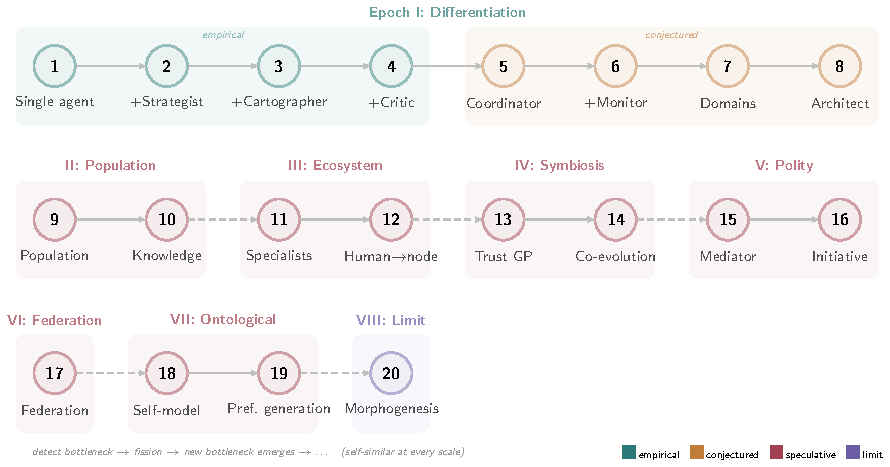
\includegraphics[width=\textwidth]{figures/teaser.pdf}
\caption{Twenty phases of architectural morphogenesis across eight epochs, graded by epistemic status: observed in the Wallfacer experiment (teal), conjectured from the fission principle (orange), speculatively extended to populations and self-reference (red), and the limiting claim that the stable attractor is morphogenesis itself (purple). Each transition is driven by bottleneck migration: resolving one constraint reliably exposes the next. The dotted loop from Phase~20 back to Phase~1 marks the claim that the entire sequence recurs at higher orders of abstraction.}
\label{fig:teaser}
\end{teaserfigure}

\maketitle

\section{Introduction}

Autonomous agentic AI systems, pipelines of LLM-based agents that plan, execute, document, verify, and sometimes deploy their own work, create a practical version of a classical epistemic problem. When one agent produces code and another agent reviews it, neither judgment supplies an unquestionable ground of correctness. The verification regress, known in philosophy as Agrippa's trilemma or M\"unchhausen's trilemma \cite{sextus_empiricus,albert1985}, therefore becomes an engineering question: how should an agentic system be structured when no component can be treated as an infallible verifier?

Most current work on LLM agents studies performance under a fixed architecture: a given role decomposition, prompting strategy, tool interface, or benchmark task is evaluated for short-horizon success \cite{li2023camel,wu2024autogen,hong2023metagpt,qian2024chatdev,yang2024sweagent}. Much less is known about \emph{architectural dynamics}: how role structure changes during prolonged autonomous operation, which pressures trigger that change, and whether the resulting dynamics can be modeled rather than narrated post hoc. This paper treats architecture itself as the dependent variable.

We investigate three research questions. \textbf{RQ1}: What recurrent patterns of architectural change appear when an autonomous agentic system operates for multiple days without human intervention? \textbf{RQ2}: When multiple instances begin from nearly null task specification, which aspects of their developmental trajectory converge and which diverge? \textbf{RQ3}: Can the autonomy boundary between agentic systems and human overseers be formalized in a way that supports measurement, learning, and later empirical testing?

To answer these questions, we combine two empirical studies with a formal and conceptual analysis. The \emph{Wallfacer} study is a seven-day longitudinal observation of an autonomous software-engineering pipeline that passed through four architectural configurations. The \emph{Ralph} study is a three-run replication experiment in which independent instances started from empty repositories with no seed task. From these studies we extract two empirical regularities. First, we observe \emph{bottleneck migration}: improvements in one system dimension repeatedly relocate the binding constraint to another. Second, we observe convergence-then-divergence: independent runs converge on the same task family while diverging in implementation language, specialization, and feature strategy.

The paper makes four contributions, ordered by epistemic strength. \textbf{Empirical}: we document bottleneck migration in Wallfacer and convergence-then-divergence in Ralph. \textbf{Analytic}: we propose a \emph{role-fission} hypothesis stating that architectural differentiation becomes likely when conflicting cognitive modes overrun a shared context budget. \textbf{Formal}: we model trust calibration as Gaussian Process preference learning with uncertainty-aware escalation and frame architecture search as constrained preferential Bayesian optimization \cite{chu2005,gonzalez2017}. \textbf{Programmatic}: we connect the framework to the literatures on self-adaptive software, organizational design, cybernetics, and security, and we mark missing evidence with explicit TODOs rather than treating speculative claims as established results.

Several scope conditions are important. The empirical base is small: one longitudinal Wallfacer trajectory and three Ralph runs, all on a single LLM substrate and within software-engineering tasks. The architectural transitions in Wallfacer were adaptive interventions, not randomized treatments, so our causal language is intentionally cautious. Accordingly, the paper should be read as a hypothesis-generating systems study plus a formal research agenda, not as a definitive theory of all agentic systems.

The remainder of the paper proceeds from observation to conjecture. Sections~2 and~3 report the Wallfacer and Ralph experiments. Section~4 extracts the role-fission principle and its falsifiable implications. Section~5 formalizes bottleneck migration, trust calibration, and architecture search. Sections~6 and~7 extend the framework into more speculative territory while keeping epistemic status explicit. Sections~8 and~9 position the work relative to prior literature, enumerate threats to validity and missing experiments, and conclude.

\section{The Wallfacer Experiment}

\subsection{Motivation and Setup}

The experiment was motivated by a straightforward question: what happens when an LLM-based agent pipeline is left to operate autonomously for an extended period? While single-turn and short-session evaluations of LLM agents are common in the literature, sustained autonomous operation over days or weeks remains underexplored. We sought to observe, rather than prescribe, the architectural pressures that emerge at scale.

The Wallfacer pipeline was deployed on a virtual private server running Ubuntu, with Claude Code \cite{anthropic2024claude} as the base LLM substrate. The pipeline was configured for a software engineering task: maintaining and extending a moderately complex codebase. It operated in a self-directed loop encompassing ideation (selecting the next task), implementation (writing code), testing (running the test suite), documentation (updating project records), and deployment (committing and pushing changes). No human reviewed or intervened in any of these stages for the duration of the experiment.

We conducted the experiment across four successive architectural configurations, each introduced when the preceding configuration exhibited sustained performance degradation that we judged, in retrospect, to stem from a structural rather than parametric limitation. The four configurations were: (1) a single agent performing all functions in a self-loop; (2) a Strategist agent separated from an Executor agent; (3) the addition of a Cartographer agent; and (4) the further addition of a Critic agent.\footnote{We name these roles after their cognitive mode rather than their mechanical function. The Strategist decides \emph{what} to do (not merely ``proposes''), the Executor implements (not merely ``builds''), the Cartographer produces legible abstractions of system state (not merely ``documents''), and the Critic exercises evaluative judgment (not merely ``verifies''). These names reflect the fission principle's emphasis on competing cognitive modes.} Each configuration was run until we observed a clear and persistent bottleneck, at which point we introduced the next configuration. The total duration across all configurations was seven days, during which the codebase grew from approximately 10,000 to over 40,000 lines of code.

\subsection{Observations and Analysis}

\begin{figure*}[t]
\centering
\begin{tikzpicture}[
    agent/.style={rectangle, rounded corners=3pt, draw=#1!70, fill=#1!12, minimum width=1.3cm, minimum height=0.55cm, font=\scriptsize\sffamily, inner sep=2pt, align=center},
    agent/.default={cBuilder},
    phase/.style={font=\small\sffamily\bfseries, text=black!80},
    bottleneck/.style={font=\tiny\sffamily\itshape, text=cBottleneck, align=center},
    arr/.style={-{Stealth[length=4pt]}, thick, black!50},
    farr/.style={-{Stealth[length=3pt]}, thick, dashed, black!35},
    trans/.style={-{Stealth[length=5pt]}, very thick, black!20},
]

\def\sep{3.8}

% Phase 1
\node[phase] at (0, 2.5) {Phase 1};
\node[agent=cBuilder, minimum width=2cm] (b1) at (0, 1.5) {Executor\\[-1pt]{\tiny(all functions)}};
\draw[arr, looseness=5] (b1.160) to[out=110,in=70] (b1.20);
\node[bottleneck] at (0, 0.3) {context\\[-1pt]competition};

\draw[trans] (1.2, 1.0) -- (\sep-1.2, 1.0);

% Phase 2
\node[phase] at (\sep, 2.5) {Phase 2};
\node[agent=cProposer] (p2) at (\sep, 2.0) {Strategist};
\node[agent=cBuilder] (b2) at (\sep, 1.0) {Executor};
\draw[arr] (p2.south) -- (b2.north);
\draw[farr] (b2.west) to[out=170,in=190] (p2.west);
\node[bottleneck] at (\sep, 0.3) {knowledge\\[-1pt]decay};

\draw[trans] (\sep+1.4, 1.5) -- (2*\sep-1.4, 1.5);

% Phase 3
\node[phase] at (2*\sep, 2.5) {Phase 3};
\node[agent=cProposer] (p3) at (2*\sep-0.9, 2.0) {Strategist};
\node[agent=cBuilder] (b3) at (2*\sep+0.9, 2.0) {Executor};
\node[agent=cDocumenter] (d3) at (2*\sep, 0.85) {Cartographer};
\draw[arr] (p3) -- (b3);
\draw[arr] (b3.south) -- (d3.north east);
\draw[farr] (d3.north west) -- (p3.south);
\node[bottleneck] at (2*\sep, 0.1) {quality\\[-1pt]control};

\draw[trans] (2*\sep+1.4, 1.5) -- (3*\sep-1.4, 1.5);

% Phase 4
\node[phase] at (3*\sep, 2.5) {Phase 4};
\node[agent=cProposer] (p4) at (3*\sep-0.9, 2.0) {Strategist};
\node[agent=cBuilder] (b4) at (3*\sep+0.9, 2.0) {Executor};
\node[agent=cDocumenter] (d4) at (3*\sep-0.9, 0.85) {Cart.};
\node[agent=cVerifier] (v4) at (3*\sep+0.9, 0.85) {Critic};
\draw[arr] (p4) -- (b4);
\draw[arr] (b4.south) -- (v4.north);
\draw[arr] (v4) -- (d4);
\draw[farr] (d4.north) -- (p4.south);
\draw[farr, cVerifier!60] (v4.east) to[out=0,in=0,looseness=1.8] (b4.east);
\node[bottleneck] at (3*\sep, 0.1) {coordination\\[-1pt]overhead};

% Bottom annotation
\draw[decorate, decoration={brace, amplitude=5pt, mirror}, thick, black!30] (-1.3, -0.3) -- (3*\sep+1.3, -0.3);
\node[font=\tiny\sffamily\itshape, text=black!50] at (1.5*\sep, -0.8) {Empirically observed in the Wallfacer experiment};

\end{tikzpicture}
\caption{Architectural evolution across four observed phases. Each transition was triggered by a persistent bottleneck (shown in red). Solid arrows indicate primary information flow; dashed arrows indicate feedback.}
\label{fig:phases}
\end{figure*}

We report three principal observations from the experiment, along with our interpretation of each. We acknowledge that as a single case study, these observations are suggestive rather than conclusive, and that alternative interpretations are possible.

\textbf{Observation 1: Bottleneck migration.} Across all four configurations, resolving a performance bottleneck in one dimension of system behavior reliably relocated the binding constraint to a different dimension, rather than producing an overall improvement that persisted. For example, in the two-agent configuration, separating planning from implementation eliminated the context-competition bottleneck observed in the single-agent configuration, but introduced a new bottleneck: implicit knowledge generated during implementation (such as the rationale behind design decisions) was not captured in any durable form and therefore decayed between planning cycles. The Cartographer was introduced to address this decay, which it did, but at the cost of introducing a quality-control bottleneck: three agents were producing outputs, but none was tasked with evaluating whether those outputs met any standard of correctness.

This pattern, in which resolving one constraint exposes another, aligns with Goldratt's Theory of Constraints \cite{goldratt1984}, which posits that any system has exactly one binding constraint at a time and that improving non-constraints yields no net throughput gain. It also resonates with the No Free Lunch theorems \cite{wolpert1997}, which establish that no single optimization strategy dominates across all problem instances. In our setting, the analogous claim is that no single architectural configuration dominates across all bottleneck types. We note, however, that our evidence for this claim is limited to a single system operating on a single class of tasks, and that broader empirical validation is required before any general principle can be asserted with confidence.

\textbf{Observation 2: Emergent self-diagnosis.} In the three-agent

\begin{figure}[t]
\centering
\begin{tikzpicture}[scale=0.82,
    cell/.style={minimum width=1.55cm, minimum height=0.34cm, font=\tiny\sffamily, inner sep=1pt},
    hi/.style={cell, fill=cVerifier!20, draw=cVerifier!50},
    lo/.style={cell, fill=cEmpirical!12, draw=cEmpirical!30},
    md/.style={cell, fill=cConjectured!10, draw=cConjectured!30},
    lbl/.style={font=\tiny\sffamily\bfseries, text=black!70, anchor=east},
    plbl/.style={font=\scriptsize\sffamily\bfseries, text=black!80}
]
\def\rh{0.48}
\def\cw{1.75}

\node[plbl] at (0, 0) {Ph.1};
\node[plbl] at (\cw, 0) {Ph.2};
\node[plbl] at (2*\cw, 0) {Ph.3};

\node[lbl] at (-0.9, -\rh) {Context};
\node[lbl] at (-0.9, -2*\rh) {Knowl.};
\node[lbl] at (-0.9, -3*\rh) {Quality};
\node[lbl] at (-0.9, -4*\rh) {Coord.};

\node[hi] at (0, -\rh) {\textbf{binding}};
\node[lo] at (0, -2*\rh) {};
\node[lo] at (0, -3*\rh) {};
\node[lo] at (0, -4*\rh) {};

\node[lo] at (\cw, -\rh) {};
\node[hi] at (\cw, -2*\rh) {\textbf{binding}};
\node[lo] at (\cw, -3*\rh) {};
\node[md] at (\cw, -4*\rh) {};

\node[lo] at (2*\cw, -\rh) {};
\node[lo] at (2*\cw, -2*\rh) {};
\node[hi] at (2*\cw, -3*\rh) {\textbf{binding}};
\node[md] at (2*\cw, -4*\rh) {};

\draw[-{Stealth[length=3pt]}, thick, cVerifier!60, dashed]
    (0.5, -\rh) to[out=-15, in=165] (\cw-0.5, -2*\rh);
\draw[-{Stealth[length=3pt]}, thick, cVerifier!60, dashed]
    (\cw+0.5, -2*\rh) to[out=-15, in=165] (2*\cw-0.5, -3*\rh);

\end{tikzpicture}
\caption{Bottleneck migration across phases. Dark cells mark the binding constraint; light cells indicate resolved dimensions. Dashed arrows show how each fission relocates the bottleneck.}
\label{fig:migration}
\end{figure}

\begin{figure*}[t]
\centering
\begin{tikzpicture}[x=1.5cm, y=3.2cm]
% Axes
\draw[-{Stealth[length=4pt]}, black!50] (0,0) -- (8.5,0) node[right, font=\tiny\sffamily, xshift=2pt] {Phase};
\draw[-{Stealth[length=4pt]}, black!50] (0,0) -- (0,1.18) node[above, font=\tiny\sffamily] {\%};

% Y-axis ticks
\foreach \y/\l in {0/0, 0.25/25, 0.5/50, 0.75/75, 1.0/100} {
    \draw[black!20] (0,\y) -- (8.2,\y);
    \node[left, font=\tiny\sffamily, text=black!50] at (-0.1,\y) {\l};
}

% X-axis labels
\foreach \x/\l in {1/1, 2/2, 3/3, 4/4, 5/5, 6/6, 7/7, 8/8} {
    \node[below, font=\tiny\sffamily, text=black!60] at (\x,-0.04) {\l};
}

% Empirical / conjectured boundary - subtle, no text in data area
\draw[dashed, black!20, thin] (4.5,-0.05) -- (4.5,1.02);
\node[font=\tiny\sffamily\itshape, text=black!30, anchor=north] at (2.25,-0.12) {empirical};
\node[font=\tiny\sffamily\itshape, text=black!30, anchor=north] at (6.35,-0.12) {conjectured};

% Data: Capability (teal)
\draw[cEmpirical, thick] plot coordinates {(1,0.60) (2,0.75) (3,0.85) (4,0.92) (5,0.95) (6,0.96) (7,0.98) (8,0.99)};
\foreach \x/\y in {1/0.60, 2/0.75, 3/0.85, 4/0.92, 5/0.95, 6/0.96, 7/0.98, 8/0.99} {
    \fill[cEmpirical] (\x,\y) circle (1.5pt);
}

% Data: Coordination cost (red)
\draw[cVerifier, thick] plot coordinates {(1,0.05) (2,0.15) (3,0.25) (4,0.38) (5,0.48) (6,0.52) (7,0.62) (8,0.58)};
\foreach \x/\y in {1/0.05, 2/0.15, 3/0.25, 4/0.38, 5/0.48, 6/0.52, 7/0.62, 8/0.58} {
    \fill[cVerifier] (\x,\y) circle (1.5pt);
}

% Data: Self-awareness (purple)
\draw[cCoordinator, thick] plot coordinates {(1,0.00) (2,0.00) (3,0.05) (4,0.08) (5,0.15) (6,0.30) (7,0.40) (8,0.80)};
\foreach \x/\y in {1/0.00, 2/0.00, 3/0.05, 4/0.08, 5/0.15, 6/0.30, 7/0.40, 8/0.80} {
    \fill[cCoordinator] (\x,\y) circle (1.5pt);
}

% Data: Boundary fluidity (orange)
\draw[cDocumenter, thick, densely dashed] plot coordinates {(1,0.00) (2,0.00) (3,0.00) (4,0.00) (5,0.02) (6,0.03) (7,0.04) (8,0.05)};
\foreach \x/\y in {5/0.02, 6/0.03, 7/0.04, 8/0.05} {
    \fill[cDocumenter] (\x,\y) circle (1.2pt);
}

% Data: Autonomy (blue)
\draw[cBuilder, thick, densely dashed] plot coordinates {(1,0.10) (2,0.15) (3,0.20) (4,0.25) (5,0.30) (6,0.35) (7,0.40) (8,0.50)};
\foreach \x/\y in {1/0.10, 2/0.15, 3/0.20, 4/0.25, 5/0.30, 6/0.35, 7/0.40, 8/0.50} {
    \fill[cBuilder] (\x,\y) circle (1.2pt);
}

% Data: Ontological depth (pink/monitor green)
\draw[cMonitor, thick, densely dotted] plot coordinates {(1,0.00) (2,0.00) (3,0.02) (4,0.05) (5,0.08) (6,0.12) (7,0.18) (8,0.25)};
\foreach \x/\y in {5/0.08, 6/0.12, 7/0.18, 8/0.25} {
    \fill[cMonitor] (\x,\y) circle (1.2pt);
}

% Legend
\node[font=\tiny\sffamily, anchor=west] at (0.2,1.08) {%
    \textcolor{cEmpirical}{\rule{6pt}{2pt}} Capability\quad
    \textcolor{cVerifier}{\rule{6pt}{2pt}} Coordination cost\quad
    \textcolor{cCoordinator}{\rule{6pt}{2pt}} Self-awareness\quad
    \textcolor{cBuilder}{\rule[0.3ex]{6pt}{0.4pt}\rule[0.3ex]{2pt}{0.4pt}\rule[0.3ex]{6pt}{0.4pt}} Autonomy\quad
    \textcolor{cDocumenter}{\rule[0.3ex]{6pt}{0.4pt}\rule[0.3ex]{2pt}{0.4pt}\rule[0.3ex]{6pt}{0.4pt}} Boundary fluidity\quad
    \textcolor{cMonitor}{$\cdots$} Ontological depth
};

% Annotations - right margin, outside plot area
\draw[-{Stealth[length=3pt]}, cCoordinator!50, thin] (8.6,0.88) -- (8.05,0.81);
\node[font=\tiny\sffamily, text=cCoordinator!80, anchor=west, align=left] at (8.65,0.88) {self-awareness\\[-1pt]jump};

\draw[-{Stealth[length=3pt]}, cVerifier!50, thin] (8.6,0.52) -- (8.05,0.58);
\node[font=\tiny\sffamily, text=cVerifier!80, anchor=west, align=left] at (8.65,0.52) {cost\\[-1pt]declines};

\end{tikzpicture}
\caption{System metric evolution across eight phases. Solid lines represent primary metrics (capability, coordination cost, self-awareness); dashed and dotted lines represent emergent metrics that become significant only in later phases (autonomy, boundary fluidity, ontological depth). Phases 1 to 4 are empirically grounded; Phases 5 to 8 are conjectured extrapolations. The sharp rise in self-awareness at Phase 8 reflects the Architect role's capacity for architectural self-modification. Values are normalized estimates based on the Wallfacer observations (Phases 1--4) and theoretical projections.}
\label{fig:metrics}
\end{figure*}

configuration (Strategist, Executor, Cartographer), the system proposed refactoring its own monolithic codebase at approximately 51,000 lines of code. This behavior did not emerge in the two-agent configuration at a comparable scale. We interpret this as evidence that the Cartographer role, by producing structured representations of the system's architecture and history, provided the Strategist with a legible abstraction of global system state that was otherwise unavailable. In the two-agent configuration, the Strategist's decisions were conditioned only on the current codebase and task queue, without any higher-level summary of architectural trends.

This interpretation finds support in Clark and Chalmers' Extended Mind hypothesis \cite{clark1998}, which argues that cognitive processes are not confined to the brain but extend to external artifacts that participate in reasoning. In our case, the documentation artifacts produced by the Cartographer function as external cognitive scaffolding for the Strategist: they do not merely record what has happened but actively shape what the Strategist can perceive and reason about. We are cautious, however, about overinterpreting a single instance of emergent behavior. It is possible that the refactoring proposal would have emerged eventually in the two-agent configuration at a higher line count, or that it was triggered by idiosyncratic features of the codebase rather than by the architectural difference we hypothesize.

\textbf{Observation 3: Coordination cost scaling.} As the number of agent roles increased from one to four, we observed a nonlinear increase in the volume of inter-agent communication required to maintain coherent system behavior. The four-agent configuration exhibited episodes of circular dependency, in which the Critic rejected output that the Executor had produced according to the Strategist's specification, leading to repeated revision cycles that consumed computational resources without advancing the project. This observation is consistent with Brooks' \cite{brooks1975} well-known finding that communication overhead in human teams scales quadratically with team size, and it suggests that the benefits of role differentiation are subject to diminishing returns as coordination costs accumulate. Figure~\ref{fig:metrics} traces the estimated trajectory of six system metrics across all eight phases, illustrating how capability saturates while coordination cost, self-awareness, and autonomy follow distinct growth curves.

\section{The Ralph Experiment: Convergent Evolution Without Specification}

The Wallfacer experiment demonstrates bottleneck migration and role fission within a single pipeline. A natural follow-up question is whether multiple independent instances, started from identical initial conditions, exhibit convergent or divergent evolutionary trajectories. To investigate this, we conducted a second experiment using a simpler pipeline that lacks Wallfacer's role differentiation.

\subsection{Setup}

We used \emph{ralph}, an autonomous agent pipeline that runs a three-phase loop: a \textbf{Thinker} analyzes the current project state and proposes exactly one goal for the next round; a \textbf{Worker} implements that goal; and a \textbf{Committer} stages all changes and pushes a commit. Unlike Wallfacer's multi-role architecture, ralph's loop is fixed: no Cartographer, no Critic, no fission. The pipeline persists execution history as JSON logs, enabling the Thinker to condition each new goal on the full trajectory of prior rounds.

We pointed ralph at three empty Git repositories with no seed task, no prompt, and no specification of what to build. The only input was an empty directory. Each instance used the same LLM substrate (Claude) and the same pipeline configuration. We let all three run autonomously; two completed 42 rounds and one completed 33 rounds before being stopped. Table~\ref{tab:ralph_repos} summarizes the resulting codebases.

\begin{table}[t]
\small
\caption{Three codebases generated by ralph from empty repositories with no seed task. All three independently converged on cellular automaton simulators.}
\label{tab:ralph_repos}
\begin{tabular}{@{}llrrr@{}}
\toprule
\textbf{Repository} & \textbf{Lang.} & \textbf{LOC} & \textbf{Funcs} & \textbf{Cost} \\
\midrule
Explorer   & C      & 10{,}876 & 133 & \$89.66 \\
Sandbox    & Python & 14{,}727 & 509 & \$56.87 \\
Simulator  & Python & 12{,}336 & 285 & \$57.80 \\
\bottomrule
\end{tabular}
\end{table}

\subsection{Observations}

\begin{figure}[t]
\centering
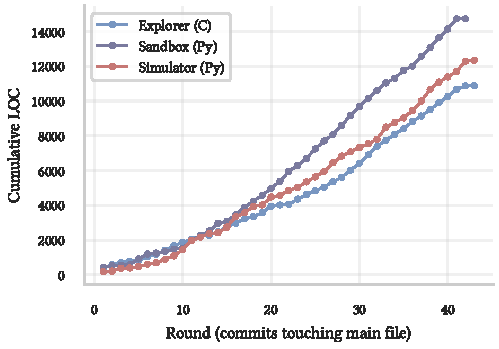
\includegraphics[width=\columnwidth]{figures/ralph_loc_growth.pdf}
\caption{Cumulative lines of code across three independently initialized repositories. All three converged on cellular automaton implementations despite receiving no seed task. Growth is monotonically increasing with near-zero churn (3.9\%, 0.5\%, and 3.0\% deletion ratios respectively).}
\label{fig:ralph_loc}
\end{figure}

\textbf{Observation 4: Convergent goal selection from null initial conditions.} All three instances independently chose to build a cellular automaton simulator as their first goal and continued developing it for every subsequent round. This convergence occurred without any seed task, prompt engineering, or inter-instance communication. The ``null'' initial condition is, of course, not truly null: it includes the LLM's entire training distribution, which implicitly encodes priors over what constitutes an interesting, tractable, and self-contained software project. The convergence on cellular automata suggests that this class of programs occupies a strong attractor basin in the LLM's prior over generative tasks --- likely because cellular automata are well-represented in training data, produce visually compelling output, and admit incremental extension without architectural refactoring. This parallels convergent evolution in biology, where independent lineages arrive at similar solutions (e.g., camera eyes evolving independently over 40 times \cite{land2002}) when facing analogous selection pressures.

\begin{figure*}[t]
\centering
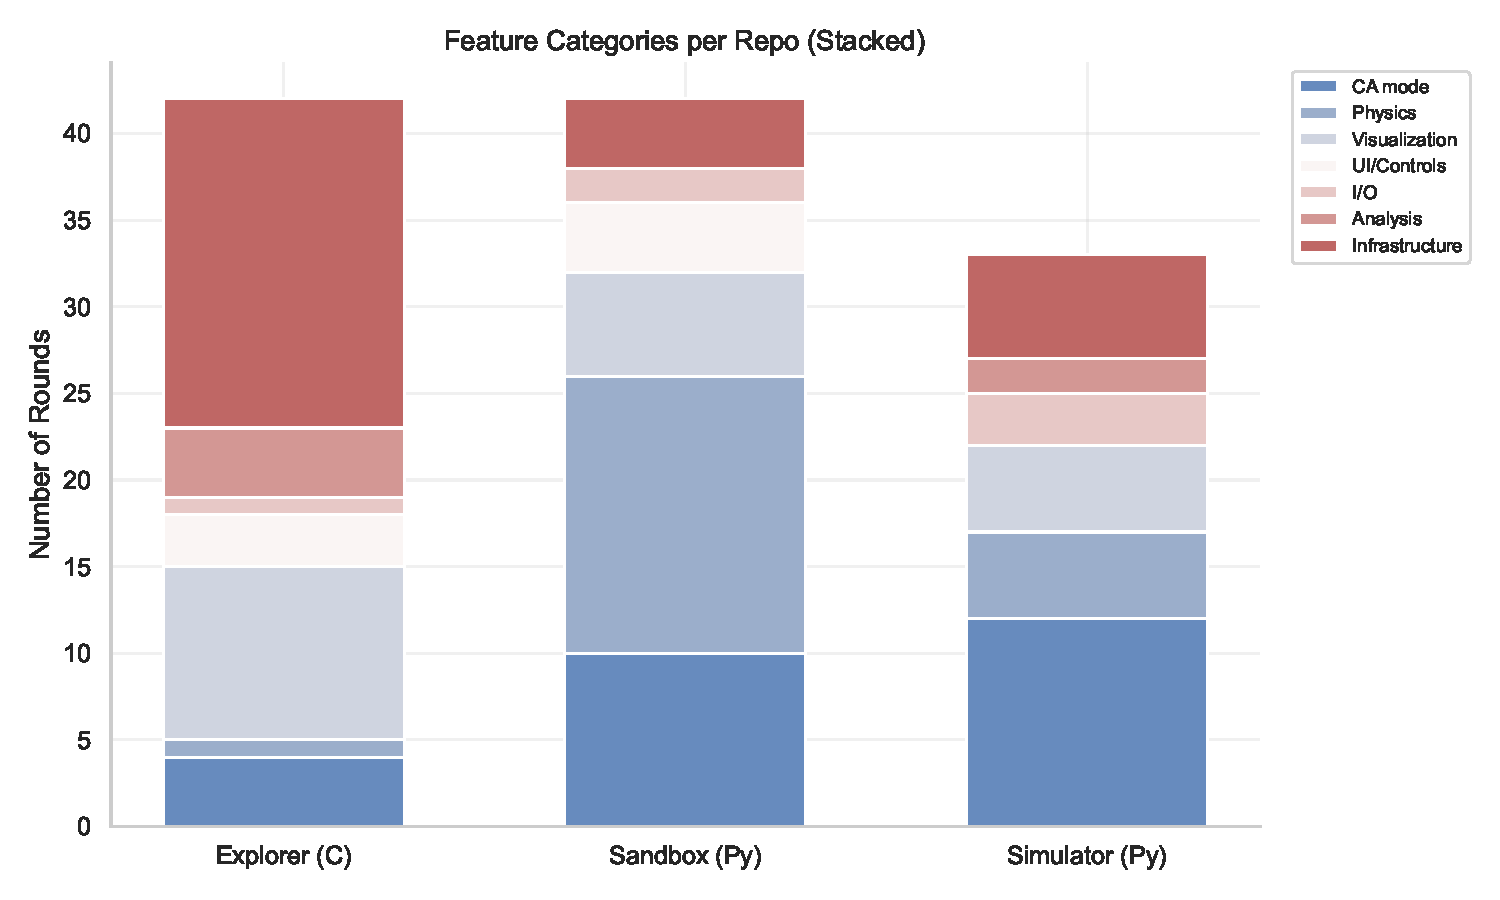
\includegraphics[width=\textwidth]{figures/ralph_feature_categories.pdf}
\caption{Feature categories per repository, classified by keyword matching on each round's Thinker goal. Despite convergent initial goals, the three codebases diverged along orthogonal axes: Explorer toward infrastructure and visualization overlays, Sandbox toward physics simulations and CA rule variants, Simulator toward CA modes and I/O capabilities.}
\label{fig:ralph_features}
\end{figure*}

\textbf{Observation 5: Divergent specialization along orthogonal axes.} Despite identical starting conditions and convergent initial goals, the three codebases specialized in qualitatively different directions (Figure~\ref{fig:ralph_features}). Explorer, written in C, developed deep scientific analysis capabilities: 15+ information-theoretic overlays (Shannon entropy, Lyapunov exponents, transfer entropy, Wolfram classification), multi-rule zones, wormhole portals, and exotic topologies (torus, Klein bottle, M\"obius strip). Sandbox pursued breadth, accumulating 27 interactive simulation modes spanning five categories (cellular automata, physics, biology, procedural generation, algorithms). Simulator combined algorithmic diversity with tooling: 28+ simulation modes alongside genetic algorithm rule discovery, headless batch rendering, and GIF/PNG export.

\begin{figure*}[t]
\centering
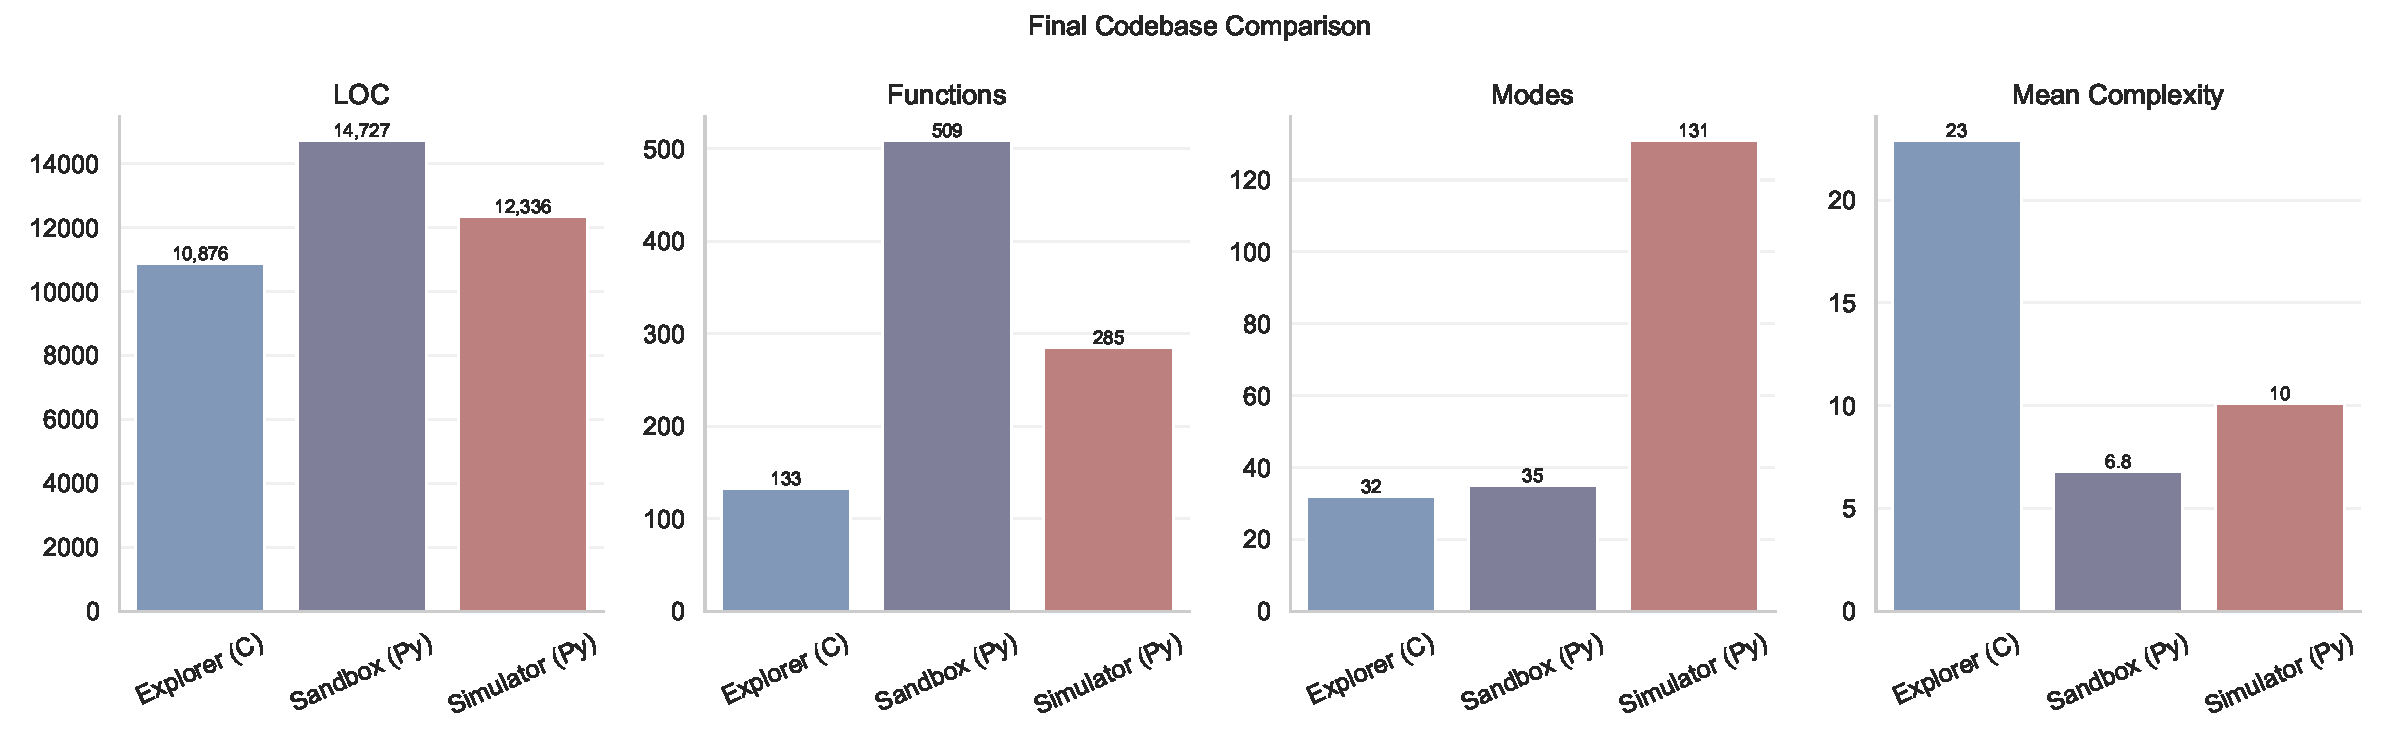
\includegraphics[width=\textwidth]{figures/ralph_final_metrics.pdf}
\caption{Final codebase comparison across four metrics. The Explorer's high mean cyclomatic complexity (22.9 vs.\ 6.8 and 10.1) reflects its C implementation and deeply nested analysis routines. The Simulator's mode count (131) dwarfs the others, reflecting its strategy of adding many small simulation variants.}
\label{fig:ralph_metrics}
\end{figure*}

Figure~\ref{fig:ralph_metrics} quantifies this divergence. The Explorer's mean cyclomatic complexity (22.9) is over three times that of the Sandbox (6.8), reflecting both the inherent verbosity of C and the depth of its analysis routines. The Simulator accumulated the most simulation modes (131) despite having the fewest rounds (33), suggesting a strategy of adding many small, self-contained variants rather than deepening existing ones. This pattern of convergence-then-divergence is consistent with adaptive radiation in evolutionary biology \cite{schluter2000}: a population that enters a new ecological zone (here, the ``cellular automaton niche'') initially exploits the same resources before diverging into specialized sub-niches.

\textbf{Observation 6: Monotonic growth without self-initiated refactoring.} Figure~\ref{fig:ralph_loc} shows that all three codebases grew monotonically, with deletion ratios below 4\%. None of the three instances ever proposed refactoring its own codebase, in contrast with the Wallfacer experiment's Observation~2, where the three-agent configuration proposed refactoring at approximately 51{,}000 lines. We interpret this as negative evidence supporting the fission principle: ralph's fixed thinker-worker-committer loop lacks a Cartographer role that would produce the structured self-representation needed for architectural self-awareness. Without a legible abstraction of global system state, the Thinker's planning horizon remains local --- it can propose the next feature but cannot diagnose structural debt. This suggests that self-diagnostic capability is an emergent property of role differentiation, not an intrinsic capability of the underlying LLM.

\section{The Fission Principle}

The observations reported above suggest a regularity that we formalize as follows.

\begin{principle}[Role Fission]
Role fission occurs when a single agent is required to simultaneously serve two cognitive modes that compete for context window resources. The fission event separates these modes into distinct agents, each with a dedicated context allocation and a narrower scope of responsibility.
\end{principle}

The three fission events observed in the Wallfacer experiment correspond to three specific mode conflicts, summarized in Table~\ref{tab:fission}.

\begin{table}[h]
\small
\caption{Observed fission events and their triggering mode conflicts.}
\label{tab:fission}
\begin{tabular}{@{}lll@{}}
\toprule
\textbf{Mode Conflict} & \textbf{Fission Product} & \textbf{Ph.} \\
\midrule
Planning vs. Implementation & Strategist & 2 \\
Execution vs. Reflection & Cartographer & 3 \\
Generation vs. Judgment & Critic & 4 \\
\bottomrule
\end{tabular}
\end{table}

This pattern bears a structural resemblance to organizational fission in human enterprises. A startup begins with a single individual performing all functions; as the enterprise grows, product management separates from engineering, technical writing separates from development, and quality assurance separates from production. Conway's Law \cite{conway1968} observes that the structure of a software system tends to mirror the communication structure of the organization that produces it. In the Wallfacer experiment, we observe a form of reverse Conway's Law: it is not organizational structure that constrains system architecture, but rather capability pressure within the system that drives structural differentiation. We note that Malone and Crowston's \cite{malone1994} coordination theory provides a formal account of how dependencies between activities give rise to coordination mechanisms, and Simon's \cite{simon1962} theory of near-decomposable systems explains why decomposition along the axis of weakest coupling tends to produce stable hierarchies.

\subsection{Theoretical Extension: Phases 5 to 8}

Beyond the four phases directly observed in the experiment, we conjecture that continued operation would produce additional fission events driven by new categories of bottleneck. We present these as theoretical predictions, not as empirical findings.

We hypothesize that the four-agent system would eventually require a \emph{Coordinator} role to manage global tradeoffs (e.g., when to refactor vs. when to add features), because no existing agent is tasked with cross-cutting prioritization. A \emph{Monitor} role may subsequently separate from the Coordinator to address context saturation, compressing raw agent outputs into summary health metrics and thereby addressing the span-of-control problem identified by Gulick \cite{gulick1937}. As system scale increases further, we anticipate domain decomposition into parallel sub-pipelines, each with its own agent stack, and eventually the emergence of an \emph{Architect} role that treats the system's own architecture as an optimization variable.

This last conjecture, that architecture becomes a variable rather than a constant, is the bridge to the formal framework developed in the next section. Whether these specific phases would materialize in practice, and in this particular order, is an empirical question that we cannot answer from the present case study.

\section{Formalization}

\subsection{Trust Calibration as Preference Learning}

The relationship between an agentic system and its human overseers can be understood as a trust calibration problem: for which decisions should the system proceed autonomously, and for which should it consult a human? Static policies (e.g., ``always consult before deployment'') are suboptimal because they either waste human attention on routine decisions or fail to escalate genuinely risky ones. We propose instead that the trust boundary should be \emph{learned} from the history of autonomous and human-assisted decisions and their outcomes.

Let $\mathcal{X}$ denote a decision context space encoding task features, system state, and environmental conditions. We define a latent trust function $f: \mathcal{X} \to \mathbb{R}$ such that $f(x)$ represents the expected relative value of autonomous operation versus human consultation at context $x$. We place a Gaussian Process prior:
\begin{equation}
f \sim \mathcal{GP}(\mu_0, k)
\end{equation}
where $\mu_0$ encodes a conservative default (consult the human when uncertain) and the kernel $k: \mathcal{X} \times \mathcal{X} \to \mathbb{R}$ encodes coherence assumptions: that similar decision contexts should yield similar trust levels, and that trust varies smoothly in the relevant features.

Crucially, we assume that observations take the form of pairwise preferences rather than scalar evaluations:
\begin{equation}
x_i \succ x_j \iff \text{outcome at } x_i \text{ preferred to outcome at } x_j
\end{equation}
This is a realistic assumption because stakeholders can typically judge that one system configuration performed better than another, even when they cannot assign absolute quality scores. Following Chu and Ghahramani \cite{chu2005}, the likelihood of an observed preference is modeled via a probit link:
\begin{equation}
P(x_i \succ x_j \mid f) = \Phi\!\left(\frac{f(x_i) - f(x_j)}{\sqrt{2}\,\sigma}\right)
\end{equation}
where $\Phi$ is the standard normal CDF and $\sigma$ captures noise in preference judgments.

The resulting posterior $p(f \mid \mathcal{D})$ constitutes a calibrated, context-dependent trust model. Its mean yields a dynamic HITL boundary: contexts where the posterior is high proceed autonomously, while contexts where it is low or uncertain trigger human consultation.

\begin{figure}[t]
\centering
\begin{tikzpicture}[scale=0.92]
% Axes
\draw[-{Stealth[length=4pt]}, thick, black!60] (0,0) -- (5.8,0) node[right, font=\tiny\sffamily] {Decision context $x$};
\draw[-{Stealth[length=4pt]}, thick, black!60] (0,-0.8) -- (0,3.2) node[above, font=\tiny\sffamily] {$f(x)$};

% GP mean curve
\draw[thick, blue!70] plot[smooth, tension=0.7] coordinates {(0.2,0.8) (1,2.2) (2,2.5) (2.8,1.8) (3.5,0.4) (4.2,1.0) (5,2.1) (5.5,2.4)};

% Confidence band
\fill[blue!8, opacity=0.6] plot[smooth, tension=0.7] coordinates {(0.2,0.3) (1,1.5) (2,1.9) (2.8,1.0) (3.5,-0.3) (4.2,0.2) (5,1.5) (5.5,1.9)} -- plot[smooth, tension=0.7] coordinates {(5.5,2.9) (5,2.7) (4.2,1.8) (3.5,1.1) (2.8,2.6) (2,3.1) (1,2.9) (0.2,1.3)} -- cycle;

% Threshold line
\draw[dashed, red!60, thick] (0, 1.4) -- (5.8, 1.4);
\node[font=\tiny\sffamily, text=red!70, anchor=west] at (5.8, 1.4) {$\tau$};

% Autonomous zone
\node[font=\tiny\sffamily, text=blue!60, fill=white, inner sep=1pt] at (1.5, 2.8) {Autonomous};

% Human zone
\node[font=\tiny\sffamily, text=red!60, fill=white, inner sep=1pt] at (3.5, -0.5) {Consult human};

% Observation points
\foreach \x/\y in {0.8/2.1, 1.5/2.4, 2.3/2.3, 3.0/1.6, 3.8/0.5, 4.5/1.1, 5.2/2.2} {
    \fill[black!70] (\x, \y) circle (1.2pt);
}

% Labels
\node[font=\tiny\sffamily, text=black!50] at (2.8, -0.7) {high risk / novel};
\node[font=\tiny\sffamily, text=black!50] at (1.2, -0.7) {routine};

\end{tikzpicture}
\caption{Conceptual illustration of the Trust GP. The blue curve shows the posterior mean of $f(x)$; the shaded band shows posterior uncertainty. The dashed threshold $\tau$ defines the HITL boundary: the system operates autonomously when $f(x) > \tau$ and consults a human otherwise. Dots represent observed preference pairs. High-uncertainty regions (e.g., novel contexts around $x \approx 3.5$) fall below the threshold even if the mean is moderate.}
\label{fig:trustgp}
\end{figure}

We observe that this formulation unifies the three classical responses to the verification regress. The kernel $k$ encodes \emph{coherentist} assumptions about which contexts should behave similarly. The observed preference pairs provide \emph{pragmatic} grounding in actual outcomes. And the posterior synthesizes both, avoiding the need for \emph{foundationalist} axioms about which verifier is ultimately authoritative. This synthesis connects to de Finetti's \cite{definetti1937} coherence conditions, Ramsey's \cite{ramsey1926} account of subjective probability, and Friston's \cite{friston2010} Free Energy Principle.

\subsection{Architecture Search as Preferential Bayesian Optimization}

If we accept the conjecture that architecture eventually becomes a variable (Phase 8), the Architect agent faces an optimization problem over a configuration space $\mathcal{C}$ encoding the number and types of agent roles, pipeline topology, and resource allocation. The objective, ``system health,'' is inherently multi-dimensional (encompassing complexity growth rate, defect rate, delivery velocity, and human satisfaction) and resists meaningful scalarization.

Preferential Bayesian Optimization (PBO) \cite{gonzalez2017} provides a natural framework: we place a GP prior over $\mathcal{C}$ and update it via preference observations of the form ``configuration $c_i$ produced better outcomes than $c_j$ under workload $w$.'' This approach differs from Neural Architecture Search \cite{zoph2017,elsken2019} in that NAS assumes a scalar reward, while PBO requires only ordinal comparisons. Whether PBO is tractable over realistic agentic configuration spaces, and whether human stakeholders can provide reliable preference judgments at this level of abstraction, are open empirical questions.

\section{Theoretical Extensions}

\begin{figure*}[t]
\centering
\begin{tikzpicture}[
    phase/.style={rounded rectangle, draw=black!50, minimum width=1.5cm, minimum height=0.55cm, font=\tiny\sffamily, inner sep=2pt},
    emp/.style={phase, fill=cEmpirical!15},
    conj/.style={phase, fill=cConjectured!10, draw=cConjectured!40},
    spec/.style={phase, fill=cSpeculative!10, draw=cSpeculative!40},
    epoch/.style={font=\tiny\sffamily\bfseries, text=black!60},
    arr/.style={-{Stealth[length=3pt]}, thick, black!30},
    every node/.style={align=center}
]

% Empirical phases
\node[emp] (p1) at (0, 0) {Ph.1\\Executor};
\node[emp] (p2) at (2.2, 0) {Ph.2\\+Strategist};
\node[emp] (p3) at (4.4, 0) {Ph.3\\+Cartographer};
\node[emp] (p4) at (6.6, 0) {Ph.4\\+Critic};

\draw[arr] (p1) -- (p2);
\draw[arr] (p2) -- (p3);
\draw[arr] (p3) -- (p4);

% Conjectured phases
\node[conj] (p5) at (8.8, 0) {Ph.5\\Coordinator};
\node[conj] (p6) at (10.6, 0) {Ph.6\\Monitor};
\node[conj] (p7) at (12.4, 0) {Ph.7\\Domains};
\node[conj] (p8) at (14.2, 0) {Ph.8\\Architect};

\draw[arr] (p4) -- (p5);
\draw[arr] (p5) -- (p6);
\draw[arr] (p6) -- (p7);
\draw[arr] (p7) -- (p8);

% Speculative extensions (below, aligned under conjectured)
\node[spec] (pe1) at (8.8, -1.4) {Population\\dynamics};
\node[spec] (pe2) at (10.6, -1.4) {Multi-\\principal};
\node[spec] (pe3) at (12.4, -1.4) {Co-\\evolution};
\node[spec] (pe4) at (14.2, -1.4) {Self-\\reference};

\draw[arr, cConjectured!50] (p8.south) -- (pe4.north);
\draw[arr, cSpeculative!40] (pe1) -- (pe2);
\draw[arr, cSpeculative!40] (pe2) -- (pe3);
\draw[arr, cSpeculative!40] (pe3) -- (pe4);

% Epoch labels
\draw[decorate, decoration={brace, amplitude=4pt}, thick, cEmpirical!50] (-0.8, 0.55) -- (7.4, 0.55);
\node[epoch, text=cEmpirical!70] at (3.3, 1.0) {Empirically observed};

\draw[decorate, decoration={brace, amplitude=4pt}, thick, cConjectured!60] (8.0, 0.55) -- (15.0, 0.55);
\node[epoch, text=cConjectured!80] at (11.5, 1.0) {Theoretically conjectured};

\draw[decorate, decoration={brace, amplitude=4pt, mirror}, thick, cSpeculative!50] (8.0, -1.95) -- (15.0, -1.95);
\node[epoch, text=cSpeculative!70] at (11.5, -2.35) {Speculative extensions};

% Driving force annotation
\node[font=\tiny\sffamily\itshape, text=black!40] at (3.3, -0.7) {Each arrow = bottleneck migration triggers fission};

\end{tikzpicture}
\caption{Roadmap of the framework's progression, with explicit epistemic grading. Blue phases (1 to 4) were directly observed in the Wallfacer experiment. Orange phases (5 to 8) are theoretically conjectured based on the fission principle. Red phases represent speculative extensions to populations, multi-stakeholder settings, and self-referential dynamics. Each transition is driven by bottleneck migration.}
\label{fig:roadmap}
\end{figure*}

The framework developed thus far rests on a single case study (Section 2) and a formal construction (Section 4). In this section, we extend the framework in directions that are increasingly speculative. We present these extensions not as findings but as a theoretical scaffold for future empirical investigation.

\subsection{From Single Systems to Populations}

A natural extension of Phase 8 is to consider multiple system instances running in parallel with heterogeneous configurations. In such a population, a routing mechanism could direct incoming tasks to the best-matched instance, and an Architect could gain organic preference pairs by comparing outcomes across configurations. This parallels the transition from individual learning to population-level selection in evolutionary biology \cite{holland1975}. Boyd and Richerson's \cite{boyd1985} dual-inheritance theory (genetic and cultural) suggests an analogous dual-inheritance model for agentic systems: architectural configuration as the ``genetic'' channel and accumulated knowledge as the ``cultural'' channel.

A shared knowledge layer across instances, which we term a Knowledge Commons, would allow learning to propagate across the population without requiring each instance to rediscover the same patterns. Henrich's \cite{henrich2004} demographic model of cultural evolution predicts that larger populations maintain more complex cultural knowledge; if this analogy holds, agent populations with shared knowledge should exhibit qualitative capability gains relative to isolated instances. However, shared knowledge also introduces the risk of \emph{knowledge pollution}, in which an erroneous belief propagated from one instance infects others, analogous to misinformation cascades in social networks \cite{vosoughi2018}.

\subsection{Multi-Principal Preference Aggregation}

In realistic deployment scenarios, multiple human stakeholders with potentially conflicting preferences interact with the system simultaneously. Arrow's impossibility theorem \cite{arrow1951} establishes that no preference aggregation function simultaneously satisfies a set of desirable axioms (unrestricted domain, Pareto efficiency, independence of irrelevant alternatives, and non-dictatorship). This result suggests that the system should not attempt to compute a single ``optimal'' configuration but should instead maintain and present a Pareto front over the multi-dimensional outcome space \cite{emmerich2006}, allowing human principals to navigate the tradeoff structure themselves.

A further speculative step concerns \emph{emergent initiative}: the possibility that a sufficiently capable system might detect cross-domain patterns invisible to any individual human principal and propose unsolicited changes. This would represent a transition from tool to collaborator, but it immediately raises legitimacy questions about authorization and accountability that connect to ongoing debates about AI alignment \cite{gabriel2020}. We raise this possibility not to endorse it but to identify it as a critical frontier for both technical and normative investigation.

\subsection{Co-evolution and Preference Generation}

If the system's outputs shape its human principals' preferences (by expanding what they consider possible), while the principals' evolving preferences shape the system's behavior, then the two are engaged in co-evolution. This mirrors niche construction in evolutionary biology \cite{odling-smee2003}, in which organisms modify their environment, altering the selection pressures that act on subsequent generations. In such a regime, neither system nor principals converge to a static equilibrium; the dynamic relationship is itself the stable attractor.

At the most speculative extreme, the GP posterior over preference space permits extrapolation into unobserved regions, enabling the system to propose preference hypotheses that its human principals have not yet articulated. Both acceptance and rejection of such proposals constitute informative signal for posterior updates. This idea resonates with Dewey's \cite{dewey1939} pragmatist account of preferences as constructed through inquiry, and with Sen's \cite{sen1977} critique of revealed preference theory. Whether such preference generation is technically feasible, epistemically legitimate, or socially desirable remains entirely open.

\section{Ontological Limits}

\subsection{Morphogenesis as the Stable Attractor}

Reviewing the progression from Phases 1 through the speculative extensions, we arrive at what we consider the paper's central theoretical claim. If the pattern of bottleneck migration is genuine (an empirical question), and if it persists at higher levels of architectural complexity (a conjecture), then the system's long-term trajectory is not toward any particular fixed architecture but toward a sustained capacity for architectural change. The cycle of detecting a bottleneck, fissioning a role, and observing the emergence of a new bottleneck would repeat at every scale: within individual agent roles, across pipelines, across populations, and at the meta-architectural level.

This characterization aligns with Prigogine and Nicolis' \cite{prigogine1977} theory of dissipative structures: systems maintained far from thermodynamic equilibrium through continuous flows of energy or information. The agentic ecosystem, on this view, persists not despite its continuous reorganization but because of it. If bottlenecks cease to migrate, the system has reached equilibrium, which in this context would indicate stagnation. The connection to Friston's \cite{friston2010} Free Energy Principle is also suggestive: the Architect's self-model functions as a generative model of the system, bottleneck detection corresponds to surprise minimization, and role fission corresponds to active inference. We stress, however, that these are analogies, not demonstrations; whether the mathematical structure of dissipative systems or free energy minimization actually applies to agentic architectures is a question for future formal analysis.

\subsection{Self-Reference and Incompleteness}

If a system constructs an explicit model of its own capabilities and limitations (as we hypothesize for Phase 8 and beyond), it enters a self-referential regime that can be analyzed using two classical results. Lawvere's fixed-point theorem \cite{lawvere1969} guarantees that in any cartesian closed category with a point-surjective morphism $\varphi: A \to B^A$, every endomorphism $f: B \to B$ has a fixed point. A verifier that verifies itself is precisely such a fixed point. Lawvere's theorem establishes that such fixed points exist in any sufficiently rich formal setting; the question is not whether self-referential equilibria are possible but what properties they have. G\"odel's first incompleteness theorem \cite{godel1931} constrains the answer: any self-model powerful enough to be useful is necessarily incomplete. The system can know that it has blind spots but cannot enumerate all of them from within.

Taken together, these results suggest that self-reconfiguring agentic systems can achieve stable but irreducibly partial self-understanding. This connects to Hofstadter's \cite{hofstadter1979} theory of strange loops, Yanofsky's \cite{yanofsky2003} unified treatment of self-referential paradoxes, and Barwise and Moss's \cite{barwise1996} non-well-founded set theory. Von Foerster's \cite{vonfoerster2003} second-order cybernetics arrives at the same structure from the operational side: when an observer recursively observes its own observations, the process converges to stable \emph{eigenbehaviors}---fixed points that the system can reliably maintain, not because they have been externally certified but because they are self-consistent solutions of the recursive process. Lawvere's theorem guarantees the existence of such fixed points in any sufficiently rich formal setting; Von Foerster's framework explains how they are realized in practice through recursive interaction rather than top-down computation. We note that applying these mathematical results to engineered software systems involves a degree of analogical reasoning that may or may not survive formal scrutiny; we present them as a conceptual framework, not as a proof.

\subsection{Ontological Pluralism and the Observer}

Finally, we note three meta-level observations that bear on the framework's interpretation. First, a single system event (e.g., a role fission) can be described as ``role differentiation'' in organizational vocabulary, ``symmetry breaking'' in thermodynamic vocabulary \cite{anderson1972}, ``strategy differentiation'' in game-theoretic vocabulary \cite{maynard-smith1982}, or ``niche divergence'' in ecological vocabulary \cite{hutchinson1957}. Each description language reveals structures that the others occlude; a system described in only one vocabulary may exhibit systematic blind spots undetectable from within that vocabulary.

Second, if all components of a system are replaceable (today's LLM agent could be tomorrow's human engineer), the system's identity resides not in its substrate but in its relational structure: its information flow topology, preference constraints, and coordination protocols. This is the category-theoretic perspective on identity \cite{mac_lane1971}, and it suggests that agentic system design should prioritize protocol-level interoperability over implementation-level homogeneity.

Third, the act of describing an agentic system is itself a component of the system it describes: a researcher analyzing the Wallfacer experiment functions as a Strategist (generating hypotheses), the analysis serves as an Executor (producing formalized descriptions), and the resulting paper acts as a Cartographer (creating artifacts that inform future experimental design). This self-referential observation, anticipated by Maturana and Varela's \cite{maturana1980} concept of autopoiesis, does not invalidate the framework but does caution against treating any description of an evolving system as final.

\section{Related Work}

The framework developed here draws on and extends several established research programs.

In \textbf{organizational theory}, the fission principle recapitulates elements of Mintzberg's \cite{mintzberg1979} structural configurations (simple structure, machine bureaucracy, adhocracy) and the coordination mechanisms catalogued by Malone and Crowston \cite{malone1994}. The principal difference is temporal: in agentic systems, structural reconfiguration can occur within minutes rather than months, enabling a much faster evolutionary cycle.

In \textbf{cybernetics}, Ashby's Law of Requisite Variety \cite{ashby1956} states that a controller must possess at least as much variety as the system it regulates. Each fission event can be understood as increasing the system's regulatory variety by dedicating a channel to a dimension of variation previously handled implicitly. The Monitor role, which compresses raw signals into summary metrics, implements a version of Conant and Ashby's \cite{conant1970} Good Regulator theorem: every good regulator of a system must contain a model of that system.

In \textbf{complex adaptive systems}, Kauffman's \cite{kauffman1993} theory of self-organization at the edge of chaos in NK fitness landscapes predicts that systems with intermediate levels of epistatic coupling evolve most effectively. Our observation that optimal fission granularity depends on context window size, task complexity, and communication bandwidth is consistent with this prediction, though we have not verified the correspondence formally.

In \textbf{information security}, the verification regress has been confronted with particular urgency. Thompson's \cite{thompson1984} Turing Award lecture demonstrated that a compiler can harbor a self-propagating trojan invisible to source-level inspection---an engineering manifestation of the incompleteness results we invoke in Section~6. The Trusted Computing Base (TCB) paradigm \cite{rushby1981} responds with an explicitly foundationalist strategy: minimize the set of components that must be assumed trustworthy, then build verification chains outward (hardware root of trust $\to$ firmware $\to$ bootloader $\to$ kernel). This mirrors our conservative GP prior $\mu_0$. Decentralized alternatives such as PGP's Web of Trust and Byzantine fault-tolerant consensus \cite{lamport1982} adopt a coherentist posture: trust emerges from mutual verification among diverse parties, though collectively compromised toolchains can defeat such checks. Bug-bounty programs and penetration testing represent the pragmatist pole: trust is calibrated not by proof but by the empirical absence of successful attack, much as our Trust GP updates on outcome-based preference pairs. Modern Zero Trust Architecture \cite{rose2020} synthesizes all three strategies---hardware roots, cross-layer consistency checks, and continuous behavioral monitoring---producing a dynamic, context-dependent trust posture structurally analogous to the learned HITL boundary of Section~4.1.  TCB minimization also offers an instructive dual to our fission principle: where fission \emph{distributes} trust across differentiated roles, TCB design seeks to \emph{concentrate} the trust-critical surface into the smallest possible core.

In \textbf{multi-agent systems}, the growing literature on LLM-based multi-agent architectures has explored role assignment, communication protocols, and evaluation frameworks. Our contribution is to situate these engineering choices within a broader evolutionary and epistemological framework, connecting them to foundational results in social choice theory, Bayesian optimization, and mathematical logic.

\section{Discussion}

\subsection{Practical Implications}

For practitioners building autonomous agentic systems, the framework suggests several design heuristics, which we offer tentatively pending broader empirical validation. First, it may be advisable to begin with the simplest architecture that functions and to add roles only when bottleneck signals are clear and persistent; premature fission incurs coordination overhead without commensurate capability gain. Second, tracking the \emph{location} of bottlenecks over time may provide a more informative diagnostic of system health than monitoring any single performance metric. Third, preference comparison rather than scalar metrics may offer a more tractable and honest approach to architecture evaluation, given the multi-dimensional nature of system health. Fourth, designing for substrate independence (communicating via protocols rather than shared implementation details) enables component substitution, whether replacing one LLM with another or replacing an agent with a human, without disrupting organizational architecture. Fifth, the HITL boundary should be learnable rather than static, as human cognitive bandwidth is typically the scarcest resource in agentic deployments.

\subsection{Limitations}

This work has several significant limitations. The Wallfacer experiment is a single case study conducted with a single LLM substrate (Claude Code) on a single class of tasks (software engineering). The 51,000-line threshold at which self-diagnosis emerged may be model-specific and task-specific; we have no evidence that it represents a general phase transition. The fission principle, while consistent with our observations, has not been tested across different LLM architectures, task domains, or team configurations. The theoretical extensions in Sections 5 and 6 are speculative and should be understood as a research agenda rather than a set of validated claims. The formal connections to Lawvere's theorem, G\"odel's incompleteness, and dissipative structures are analogical rather than deductive, and it remains to be seen whether they can be made rigorous.

\subsection{Open Questions}

Several questions merit investigation. First, can a normalized complexity metric predict architectural fission thresholds across different substrates and task domains? Second, do autonomous agentic systems converge to stable configurations, oscillate, or drift unboundedly under sustained operation? The dissipative structure analogy suggests oscillation as the generic attractor, but this has not been empirically established. Third, when does role fission improve net system performance (capability gain exceeding coordination cost), and can this be connected to optimal stopping theory \cite{shiryaev2007}? Fourth, how should independent agentic ecosystems establish inter-system trust and negotiate shared protocols? MCP \cite{anthropic2024mcp} provides a communication primitive, but the trust and preference negotiation layers remain to be designed.

\section{Conclusion}

We have presented a framework for understanding the architectural evolution of autonomous agentic systems, grounded in empirical observations from the Wallfacer experiment and extended through formal and theoretical analysis. The central empirical finding, bottleneck migration, connects to established results in operations research, optimization theory, and cybernetics. The fission principle provides a candidate explanation for observed patterns of role differentiation. The formalization of trust as Gaussian Process preference learning offers a principled approach to the HITL boundary problem. The theoretical extensions to populations, multi-principal scenarios, and self-referential self-models map a large and largely unexplored conceptual space.

We conclude with what we consider the framework's most important, if most speculative, implication. If the pattern of bottleneck migration is genuine and persistent, then the long-term trajectory of agentic architecture is not toward a fixed optimal design but toward a sustained capacity for redesign. The questions practitioners and researchers pose about these systems (``How should I structure the agents?'' at one level; ``How should the system restructure itself?'' at another; ``What constitutes the system's boundary?'' at a third) themselves recapitulate the detect-fission-emerge cycle that the framework describes. Whether this self-similarity is a deep structural feature of complex adaptive systems or merely a suggestive analogy is, we believe, one of the more interesting open questions in the field.


\bibliographystyle{plainnat}
\bibliography{references}

\end{document}
